% 第8章第4节：稳定性与长期行为（平衡点、线性化与谱判据；Lyapunov函数与极限集合；持续输入下的轨迹响应）。

\section{稳定性与长期行为}
\label{sec:ode-stability}

第~\ref{sec:ode-continuous-dependence}小节的估计允许误差按$e^{Lt}$增长，只在有限时间内有用。实际关心的常常是另一类问题：房间最终是否稳定在某个温度，摆是否终将停下，微小的初值误差是越来越小还是越来越大。本节在同一个给定系统内依次研究三种情形：平衡点附近的小扰动，用谱和线性化判断；较大的区域乃至全空间，用Lyapunov函数与极限集合判断；持续存在的输入，用常数变易与含输入项的Lyapunov不等式估计状态范围。局部的线性判据与非线性的全局条件要分清，前者回答“离平衡足够近时”，后者回答“从这片区域出发时”。

本节只讨论自治方程$\dot{\bm x}=\bm g(\bm x)$，$\bm g$在开集$D$上局部Lipschitz；恒定输入已经代入$\bm g$。非自治情形需要把各项条件改为关于初始时刻一致成立，这里不展开。

\subsection{平衡点、线性化与谱判据}
\label{sec:ode-linear-stability}

\paragraph{平衡点与三种稳定}
满足$\bm g(\bm x^\ast)=\bm0$的状态$\bm x^\ast$称为\term{平衡点}（equilibrium）。从平衡点出发的解就是常值$\bm x^\ast$。温度模型在恒定加热$u$下的平衡点是$x^\ast=u/\lambda$；摆的平衡点是$(q,p)=(k\pi,0)$，偶数$k$对应摆锤在最低点，奇数$k$对应倒立。

真实系统不会恰好从平衡点出发。我们要问三件不同的事：小的初值偏差是否始终保持小；它是否最终消失；消失是否有统一的指数速度。

\begin{definition}[平衡点的稳定性]
  \label{def:ode-equilibrium-stability}
  设$\bm x^\ast$是$\dot{\bm x}=\bm g(\bm x)$的平衡点。
  \begin{enumerate}
    \item 若对每个$\varepsilon>0$存在$\delta>0$，使$\|\bm x_0-\bm x^\ast\|_2<\delta$时解对全部$t\geq0$存在并满足$\|\bm x(t)-\bm x^\ast\|_2<\varepsilon$，称$\bm x^\ast$在Lyapunov意义下\term{稳定}。
    \item 若存在$r>0$，使$\|\bm x_0-\bm x^\ast\|_2<r$时解对全部$t\geq0$存在并满足$\bm x(t)\to\bm x^\ast$，称$\bm x^\ast$是吸引的。稳定且吸引称为\term{渐近稳定}。
    \item 若存在$r,C,\alpha>0$，使$\|\bm x_0-\bm x^\ast\|_2<r$时解对全部$t\geq0$存在并满足
    \[
      \|\bm x(t)-\bm x^\ast\|_2\leq Ce^{-\alpha t}\|\bm x_0-\bm x^\ast\|_2,
    \]
    称$\bm x^\ast$\term{指数稳定}。
  \end{enumerate}
  若第2、3条对$D=\mathbb R^d$中的全部初值成立，相应地称为全局渐近稳定与全局指数稳定。不稳定指不满足第1条。
\end{definition}

这些定义都对一整个邻域里的初值下结论，并且要求解对全部未来存在；展示一条收敛的轨迹不能代替这样的量词。三个性质逐条加强，表~\ref{tab:ode-stability-types}用三个标量方程说明后一个确实比前一个多要求了东西。

\begin{table}[htbp]
  \centering
  \begin{tabular}{llll}
    \toprule
    方程 & 小偏差始终小 & 偏差趋于零 & 统一指数衰减\\
    \midrule
    $\dot x=0$ & 是，状态保持初值 & 否 & 否\\
    $\dot x=-x^3$ & 是，$|x(t)|$不增 & 是 & 否\\
    $\dot x=-x$ & 是 & 是 & 是\\
    \bottomrule
  \end{tabular}
  \caption{原点的三种稳定性质。$\dot x=-x^3$的解为$x(t)=x_0/\sqrt{1+2x_0^2t}$，按$t^{-1/2}$衰减，没有统一的指数速度；$\dot x=-x$的解为$e^{-t}x_0$。三个方程的解都对全部$t\geq0$存在。}
  \label{tab:ode-stability-types}
\end{table}

“稳定”与“吸引”控制的是不同的东西：前者限制轨迹在整个未来离平衡多远，后者只要求最终回来。所以渐近稳定的定义同时要求二者。指数稳定还要求衰减速率和常数$C$在整个邻域内统一，这一点在数值计算和输入响应估计中很重要，因为它使误差界可以写成具体的数。

\paragraph{线性系统的谱判据}
对线性系统$\dot{\bm x}=\bm A\bm x$，原点总是平衡点，并且解$e^{t\bm A}\bm x_0$关于初值线性，邻域的大小无关紧要：局部性质与全局性质相同。稳定性完全由$e^{t\bm A}$的长期行为决定，而上一节已经看到，$e^{t\bm A}$由特征值和Jordan结构决定。

\begin{theorem}[线性系统的谱判据]
  \label{thm:ode-linear-spectral-stability}
  设$\bm A\in\mathbb R^{d\times d}$。
  \begin{enumerate}
    \item $\dot{\bm x}=\bm A\bm x$的原点渐近稳定，当且仅当它全局指数稳定，当且仅当$\bm A$的全部特征值实部严格为负。这样的矩阵称为\term{Hurwitz矩阵}。
    \item 原点稳定，当且仅当全部特征值实部不大于零，并且实部为零的特征值对应的Jordan块都是$1\times1$的。
  \end{enumerate}
\end{theorem}

\begin{proof}
  在复数域写Jordan分解$\bm A=\bm V\bm J\bm V^{-1}$，于是$e^{t\bm A}=\bm Ve^{t\bm J}\bm V^{-1}$，只需对$\bm J$逐块研究。大小为$r$的块$\lambda\bm I+\bm N$的指数为$e^{\lambda t}\sum_{j<r}t^j\bm N^j/j!$，其各元素的模是$e^{t\operatorname{Re}\lambda}$乘以次数小于$r$的多项式。

  (1)若全部$\operatorname{Re}\lambda<0$，取$0<\alpha<\min_\lambda(-\operatorname{Re}\lambda)$。每个块都满足$e^{t\operatorname{Re}\lambda}t^j\leq C_je^{-\alpha t}$，有限个块合起来得$\|e^{t\bm A}\|\leq Ce^{-\alpha t}$，这就是全局指数稳定；它蕴含渐近稳定。反过来，若某个特征值$\lambda$满足$\operatorname{Re}\lambda\geq0$，取其特征向量$\bm v$，复解$e^{\lambda t}\bm v$的模不趋于零；它的实部和虚部都是实解，至少一个不趋于零，原点不是吸引的。

  (2)稳定等价于$\|e^{t\bm A}\|$在$t\geq0$上有界：有界时取$\delta=\varepsilon/\sup_t\|e^{t\bm A}\|$即可；无界时存在初值方向使解的范数任意大，按比例缩小初值也无法让它对所有$t$保持小。$\operatorname{Re}\lambda<0$的块有界；$\operatorname{Re}\lambda=0$的$1\times1$块$e^{\lambda t}$模为$1$，有界；$\operatorname{Re}\lambda=0$而块大小$r\geq2$时出现模为$t$的元素，无界；$\operatorname{Re}\lambda>0$时无界。
\end{proof}

两个判据的分界在虚轴上：严格在左半平面意味着指数衰减；落在虚轴上要看Jordan结构，可能稳定而不吸引（如中心），也可能多项式增长。例如$\bm A=\begin{bmatrix}0&1\\0&0\end{bmatrix}$的两个特征值都是零，但解$x_1(t)=x_1(0)+tx_2(0)$线性增长，原点不稳定。把严格不等号放宽成非严格不等号，结论就不再成立。

\paragraph{渐近衰减不等于单调下降}
Hurwitz条件保证$\|e^{t\bm A}\|\leq Ce^{-\alpha t}$，但常数$C$可能很大，状态在衰减之前可能先显著增长。取
\[
  \bm A=\begin{bmatrix}-1&K\\0&-2\end{bmatrix},\qquad K\geq0,
\]
特征值是$-1,-2$，与$K$无关。从$\bm x_0=(0,1)$出发，$x_2(t)=e^{-2t}$，而$x_1$满足$\dot x_1=-x_1+Ke^{-2t}$，解为$x_1(t)=K(e^{-t}-e^{-2t})$。$x_1$在$t=\log2$处达到最大值$K/4$。图~\ref{fig:ode-transient-growth}显示，$K=8$时状态范数从$1$升到约$2.02$，$K=20$时升到约$5.01$，此后才衰减。

\begin{figure*}[htbp]
  \centering
  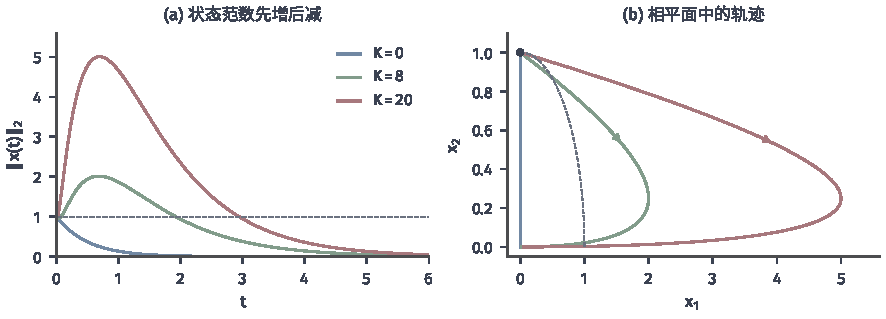
\includegraphics[width=150mm]{figures/03-optimization-evolution-and-signals/02-processes-and-trajectory-evolution/matplotlib/ode-transient-growth/figure.pdf}
  \caption{同谱系统的瞬态放大。$\bm A=\begin{bmatrix}-1&K\\0&-2\end{bmatrix}$，特征值恒为$-1,-2$，初值$(0,1)$。(a)状态的欧氏范数，$K=0,8,20$时峰值分别为$1$、约$2.02$、约$5.01$，灰色虚线为初始范数$1$。(b)相平面中的轨迹，灰色虚线为单位圆弧；$K>0$时轨迹先远离原点再返回。}
  \label{fig:ode-transient-growth}
\end{figure*}

放大来自第二个坐标向第一个坐标的单向耦合。$x_2$衰减的过程中不断向$x_1$输送“推力”，$x_1$来不及衰减就被推高。$K\neq0$时$\bm A\bm A^\top\neq\bm A^\top\bm A$，这类矩阵称为非正规矩阵；它的特征向量$(1,0)$与$(K,-1)$在$K$大时几乎共线，特征值只描述了最终的衰减速率，没有描述特征方向之间的几何关系。

何时会出现增长，可以直接从欧氏范数的导数判断：
\[
  \frac{\mathrm d}{\mathrm dt}\frac12\|\bm x\|_2^2=\bm x^\top\bm A\bm x=\bm x^\top\bm S\bm x,\qquad\bm S=\frac{\bm A+\bm A^\top}2.
\]
所以范数对一切初值都单调不增，当且仅当对称部分$\bm S$半负定。本例$\bm S$的最大特征值为$\bigl(-3+\sqrt{1+K^2}\bigr)/2$，$K>2\sqrt2$时为正，存在一些初始方向使范数先增长。谱判据说明“最终会回来”，对称部分说明“此刻是否在靠近”，二者回答的问题不同。下面的Lyapunov方程表明，换一个合适的二次型度量距离，就能让每条轨迹都单调靠近原点。

\paragraph{Lyapunov方程}
若欧氏距离不单调，不妨找一个椭圆形的度量：$V(\bm x)=\bm x^\top\bm P\bm x$，$\bm P\succ\bm0$。沿解有$\dot V=\bm x^\top(\bm A^\top\bm P+\bm P\bm A)\bm x$。要求它对一切非零$\bm x$为负，就是要求$\bm A^\top\bm P+\bm P\bm A$负定。

\begin{theorem}[连续时间Lyapunov方程]
  \label{thm:ode-lyapunov-equation}
  $\bm A$为Hurwitz矩阵，当且仅当对每个对称正定的$\bm Q$，存在唯一的对称正定$\bm P$满足
  \begin{equation}
    \bm A^\top\bm P+\bm P\bm A=-\bm Q.
    \label{eq:ode-lyapunov-equation}
  \end{equation}
\end{theorem}

\begin{proof}
  设$\bm A$为Hurwitz矩阵，令$\bm P=\int_0^\infty e^{t\bm A^\top}\bm Qe^{t\bm A}\,\mathrm dt$。由定理~\ref{thm:ode-linear-spectral-stability}，被积函数按$e^{-2\alpha t}$衰减，积分收敛。对非零$\bm x$，
  \[
    \bm x^\top\bm P\bm x=\int_0^\infty(e^{t\bm A}\bm x)^\top\bm Q(e^{t\bm A}\bm x)\,\mathrm dt>0,
  \]
  所以$\bm P\succ\bm0$。被积函数对$t$的导数是$\bm A^\top(\cdot)+(\cdot)\bm A$，积分得$\bm A^\top\bm P+\bm P\bm A=\bigl[e^{t\bm A^\top}\bm Qe^{t\bm A}\bigr]_0^\infty=-\bm Q$。若另有解，两解之差$\bm D$满足$\bm A^\top\bm D+\bm D\bm A=\bm0$，于是$\frac{\mathrm d}{\mathrm dt}\bigl(e^{t\bm A^\top}\bm De^{t\bm A}\bigr)=\bm0$，即$e^{t\bm A^\top}\bm De^{t\bm A}=\bm D$；令$t\to\infty$得$\bm D=\bm0$。

  反过来，设$\bm P,\bm Q\succ\bm0$满足方程。记$p_-,p_+$为$\bm P$的最小、最大特征值，$q_-$为$\bm Q$的最小特征值，则$p_-\|\bm x\|_2^2\leq V\leq p_+\|\bm x\|_2^2$，并且$\dot V=-\bm x^\top\bm Q\bm x\leq-q_-\|\bm x\|_2^2\leq-(q_-/p_+)V$。于是$\frac{\mathrm d}{\mathrm dt}\bigl(e^{(q_-/p_+)t}V\bigr)\leq0$，得$V(t)\leq e^{-(q_-/p_+)t}V(0)$，从而
  \[
    \|\bm x(t)\|_2\leq\sqrt{p_+/p_-}\;e^{-q_-t/(2p_+)}\|\bm x_0\|_2.
  \]
  这是全局指数稳定，由定理~\ref{thm:ode-linear-spectral-stability}，$\bm A$为Hurwitz矩阵。
\end{proof}

\begin{example}[手算Lyapunov方程]
  \label{ex:ode-lyapunov-equation}
  取$\bm A=\begin{bmatrix}0&1\\-2&-3\end{bmatrix}$，特征值$-1,-2$。令$\bm Q=\bm I$，$\bm P=\begin{bmatrix}p&q\\q&r\end{bmatrix}$，方程~\eqref{eq:ode-lyapunov-equation}的三个独立分量为$-4q=-1$、$p-3q-2r=0$、$2q-6r=-1$，解得$q=r=\tfrac14$，$p=\tfrac54$。$\bm P$的特征值约为$1.309$与$0.191$，确实正定。由上面的估计，$\|\bm x(t)\|_2$的上界按$e^{-t/(2\times1.309)}\approx e^{-0.38t}$衰减。这是一个保证，比最慢模态的真实速率$e^{-t}$保守。另一方面，$\bm A$的对称部分$\begin{bmatrix}0&-1/2\\-1/2&-3\end{bmatrix}$有正特征值约$0.081$，所以欧氏范数并非对一切初值单调下降，而$\bm P$给出的椭圆度量却是单调的。
\end{example}

图~\ref{fig:ode-lyapunov-levels}(a)画出这个例子：黄色椭圆是$V=\bm x^\top\bm P\bm x$的等值线，蓝色轨迹每穿过一条椭圆都由外向内，从不回头。线性系统因此总能为稳定的动力学找到一个二次“能量”，只是这个能量一般不是欧氏范数的平方。

\paragraph{非线性系统的局部线性化}
在平衡点附近，光滑向量场近似于它的线性部分。设$\bm g$在$\bm x^\ast$附近连续可微，记Jacobian矩阵$\bm J=\partial\bm g(\bm x^\ast)$，偏差$\bm e=\bm x-\bm x^\ast$满足
\[
  \dot{\bm e}=\bm J\bm e+\bm\rho(\bm e),\qquad\|\bm\rho(\bm e)\|_2\leq\epsilon(r)\|\bm e\|_2\quad(\|\bm e\|_2\leq r),
\]
其中$\epsilon(r)\to0$（$r\to0$），这正是可微性的定义。问题是：高阶项$\bm\rho$会不会改变线性部分给出的结论？

\begin{theorem}[线性化判据]
  \label{thm:ode-linearization}
  设$\bm g$在平衡点$\bm x^\ast$的邻域内连续可微，$\bm J=\partial\bm g(\bm x^\ast)$。
  \begin{enumerate}
    \item 若$\bm J$为Hurwitz矩阵，则$\bm x^\ast$局部指数稳定。
    \item 若$\bm J$有实部为正的特征值，则$\bm x^\ast$不稳定。
  \end{enumerate}
\end{theorem}

\begin{proof}
  (1)由定理~\ref{thm:ode-lyapunov-equation}取$\bm P\succ\bm0$满足$\bm J^\top\bm P+\bm P\bm J=-\bm I$，令$V(\bm e)=\bm e^\top\bm P\bm e$。沿解，
  \[
    \dot V=-\|\bm e\|_2^2+2\bm e^\top\bm P\bm\rho(\bm e)\leq-\bigl(1-2p_+\epsilon(r)\bigr)\|\bm e\|_2^2\qquad(\|\bm e\|_2\leq r).
  \]
  取$r$足够小，使$2p_+\epsilon(r)\leq\tfrac12$且闭球在邻域内，则$\dot V\leq-\tfrac12\|\bm e\|_2^2\leq-V/(2p_+)$。集合$\{V<p_-r^2\}$包含在半径$r$的球内；从其中出发的解，$V$沿途不增，所以不能离开这个集合，由定理~\ref{thm:ode-escape}对全部$t\geq0$存在。与上一定理的证明相同，得$\|\bm e(t)\|_2\leq\sqrt{p_+/p_-}\,e^{-t/(4p_+)}\|\bm e(0)\|_2$。

  (2)的证明构造一个在不稳定方向上增长的二次函数，论证与(1)类似但更长，这里引用其结论。
\end{proof}

第(2)条的完整证明见Khalil的非线性系统教材\scite{math-khalil2002nonlinear}。线性化给出的是局部结论：它只说明从足够近处出发的轨迹回到平衡点，不说明“足够近”有多近。若$\bm J$的特征值落在虚轴上而其余都在左半平面，线性化无法判断，高阶项决定结果。$\dot x=-x^3$与$\dot x=x^3$在原点的线性化都是$0$，前者渐近稳定，后者的解$x_0/\sqrt{1-2x_0^2t}$在有限时间爆炸，原点不稳定。

回到摆。最低点$(0,0)$处$\bm J=\begin{bmatrix}0&1\\-1&-c\end{bmatrix}$，$c>0$时为Hurwitz矩阵，最低点局部指数稳定；$c=0$时特征值为$\pm\mathrm i$，线性化无法判断，下一小节用能量说明它稳定但不吸引。倒立点$(\pi,0)$处$\bm J=\begin{bmatrix}0&1\\1&-c\end{bmatrix}$，行列式为$-1<0$，有一个正特征值，是鞍点，不稳定。这些局部画面正是图~\ref{fig:ode-phase-portraits}中的焦点、中心与鞍点。

\paragraph{虚轴与单位圆}
第~\ref{chap:discrete-dynamical-systems}章的离散线性系统$\bm x_{n+1}=\bm M\bm x_n$以单位圆为界：全部特征值的模小于$1$时渐近稳定。连续时间的界是虚轴。两者通过指数映射对应：步长为$h$的精确采样给出$\bm M=e^{h\bm A}$，其特征值为$e^{h\lambda}$，模为$e^{h\operatorname{Re}\lambda}$，于是$\operatorname{Re}\lambda<0$恰好对应$|e^{h\lambda}|<1$。精确采样保持稳定性；近似的离散化却未必。Euler近似给出$\bm M=\bm I+h\bm A$，特征值为$1+h\lambda$，它落在单位圆内要求$h\lambda$落在以$-1$为心的单位圆盘内，例如$\lambda=-0.2$时要求$h<10$。离散与连续的稳定条件不能套用同一个不等式，第~\ref{sec:ode-stiff}小节将系统研究这一点。

\subsection{Lyapunov函数与极限集合}
\label{sec:ode-lyapunov}

\paragraph{沿轨迹的变化率}
线性化只看平衡点的一个小邻域。要对更大的区域下结论，可以模仿Lyapunov方程中的做法：找一个标量函数$V$度量“离平衡有多远”，再证明它沿每条轨迹下降。关键在于不需要求出轨迹就能计算这个下降速率。若$V$连续可微，链式法则给出
\[
  \frac{\mathrm d}{\mathrm dt}V\bigl(\bm x(t)\bigr)=\nabla V\bigl(\bm x(t)\bigr)^\top\bm g\bigl(\bm x(t)\bigr).
\]
右端只依赖当前状态，于是定义$\dot V(\bm x)=\nabla V(\bm x)^\top\bm g(\bm x)$，它是$V$的梯度与向量场的内积。几何上，把$V$的等值线画在相平面上：$\dot V<0$意味着向量场在每一点都指向$V$更小的一侧，轨迹只能一层一层地穿过等值线向内走。

以原点为平衡点，称$C^1$函数$V$在原点的邻域$U$内正定，若$V(\bm0)=0$且$V(\bm x)>0$对$\bm x\in U\setminus\{\bm0\}$成立。正定只是形状上的要求，说明“$V$小”意味着“离原点近”；它还没有说明$V$沿轨迹怎样变化。

\begin{definition}[Lyapunov函数]
  \label{def:ode-lyapunov-function}
  设原点是$\dot{\bm x}=\bm g(\bm x)$的平衡点，$V$在原点的邻域$U$内连续可微且正定。若$\dot V(\bm x)\leq0$对$\bm x\in U$成立，称$V$为$U$上的\term{Lyapunov函数}；若$\dot V(\bm x)<0$对$\bm x\in U\setminus\{\bm0\}$成立，称为严格Lyapunov函数。
\end{definition}

\begin{theorem}[连续时间Lyapunov判据]
  \label{thm:ode-lyapunov}
  \label{thm:dynamical-nonlinear-lyapunov}
  设原点是$\dot{\bm x}=\bm g(\bm x)$的平衡点，$\bm g$在原点的邻域$U$内局部Lipschitz。
  \begin{enumerate}
    \item 若$U$上存在Lyapunov函数，则原点稳定。
    \item 若$U$上存在严格Lyapunov函数，则原点渐近稳定。
    \item 若$U=\mathbb R^d$，$V$在$\mathbb R^d$上正定、径向无界（即$\|\bm x\|_2\to\infty$时$V(\bm x)\to\infty$），并且$\dot V\leq0$，则每条解对全部$t\geq0$存在且原点稳定；若进而$\dot V(\bm x)<0$对一切$\bm x\neq\bm0$成立，则原点全局渐近稳定。
  \end{enumerate}
\end{theorem}

\begin{proof}
  (1)取$\varepsilon>0$足够小，使闭球$\bar B_\varepsilon=\{\|\bm x\|_2\leq\varepsilon\}\subseteq U$。$V$在球面$\|\bm x\|_2=\varepsilon$上连续且为正，有正的最小值$c_\varepsilon$。$V$在原点连续且$V(\bm0)=0$，故存在$\delta\in(0,\varepsilon)$使$\|\bm x_0\|_2<\delta$时$V(\bm x_0)<c_\varepsilon$。从这样的$\bm x_0$出发，只要轨迹留在$\bar B_\varepsilon$中，$V$就不增，始终小于$c_\varepsilon$；而要离开球，轨迹必须先到达球面，那里$V\geq c_\varepsilon$，矛盾。于是轨迹留在紧集$\bar B_\varepsilon$中，由定理~\ref{thm:ode-escape}对全部$t\geq0$存在，且$\|\bm x(t)\|_2<\varepsilon$，这就是稳定性。

  (2)沿用(1)中的轨迹。$V(\bm x(t))$单调不增且非负，有极限$v_\infty\geq0$。若$v_\infty>0$，由$V$的连续性，存在$\eta>0$使$\|\bm x(t)\|_2\geq\eta$对全部$t$成立（否则轨迹会任意接近原点，$V$也会任意接近$0$）。在紧集$\{\eta\leq\|\bm x\|_2\leq\varepsilon\}$上连续函数$-\dot V$有正的最小值$\kappa$，于是$V(\bm x(t))\leq V(\bm x_0)-\kappa t$，$t$大时为负，矛盾。故$v_\infty=0$。最后，若$\bm x(t)$不趋于零，则有$\eta'>0$与$t_j\to\infty$使$\|\bm x(t_j)\|_2\geq\eta'$，从而$V(\bm x(t_j))\geq\min_{\eta'\leq\|\bm x\|_2\leq\varepsilon}V>0$，与$v_\infty=0$矛盾。

  (3)径向无界保证每个子水平集$\{V\leq V(\bm x_0)\}$有界，它又是闭集，所以紧。轨迹的$V$不增，因而留在这个紧集中，对全部$t\geq0$存在。稳定性同(1)。严格下降时，把(2)中的球$\bar B_\varepsilon$换成这个子水平集，同样的论证对任意初值成立。
\end{proof}

为什么全局结论需要径向无界？若$V$在远处趋于一个有限值，它的某些子水平集就无界，轨迹可以一边让$V$下降，一边沿着无界的子水平集跑向无穷。只在原点附近正定，控制不了远处的状态。

\begin{example}[线性化失效而Lyapunov函数有效]
  \label{ex:ode-lyapunov-cubic}
  考虑$\dot x_1=-x_1^3+x_2$，$\dot x_2=-x_1-x_2^3$。原点的Jacobian矩阵为$\begin{bmatrix}0&1\\-1&0\end{bmatrix}$，特征值$\pm\mathrm i$，定理~\ref{thm:ode-linearization}无法判断。取$V=(x_1^2+x_2^2)/2$，则
  \[
    \dot V=x_1(-x_1^3+x_2)+x_2(-x_1-x_2^3)=-x_1^4-x_2^4,
  \]
  在原点之外严格为负；$V$正定且径向无界。由定理~\ref{thm:ode-lyapunov}，原点全局渐近稳定。衰减却不是指数的：$\dot V\geq-(x_1^2+x_2^2)^2=-4V^2$，所以$V(t)\geq V_0/(1+4V_0t)$，只按$1/t$减小。
\end{example}

若还能找到常数$c_1,c_2,c_3>0$使$c_1\|\bm x\|_2^2\leq V\leq c_2\|\bm x\|_2^2$且$\dot V\leq-c_3\|\bm x\|_2^2$，Lyapunov方程证明中的积分估计照样适用，给出指数稳定。一般的严格下降没有这种二次比较，上例就是渐近稳定而不指数稳定的情形。

\paragraph{不变集与$\omega$极限集}
许多物理系统的能量只在部分方向上耗散。阻尼摆的机械能$V=p^2/2+(1-\cos q)$满足$\dot V=-cp^2$，在整条直线$p=0$上为零，所以$V$只是非严格的Lyapunov函数，定理~\ref{thm:ode-lyapunov}的(2)用不上。可是直觉上摆终将停下：轨迹即使碰到$p=0$，也会被重力立刻推离。要把这一直觉写成证明，需要描述“轨迹最终停留在哪里”。

\begin{definition}[不变集与$\omega$极限集]
  \label{def:ode-invariant-limit-sets}
  \label{def:dynamical-invariant-limit-sets}
  设$\bm\varphi_t$是局部Lipschitz自治方程的流。
  \begin{enumerate}
    \item 若从$\Omega$中每一点出发的解对全部$t\geq0$存在且$\bm\varphi_t(\Omega)\subseteq\Omega$，称$\Omega$为\term{正向不变集}。
    \item 若从$M$中每一点出发的解对全部$t\in\mathbb R$存在且$\bm\varphi_t(M)=M$对全部$t\geq0$成立，称$M$为\term{不变集}。等价地，$M$中每一点都位于一条始终留在$M$中的完整轨迹上。
    \item 设从$\bm x_0$出发的解对全部$t\geq0$存在。它的\term{$\omega$极限集}是
    \[
      \omega(\bm x_0)=\bigl\{\bm z:\text{存在}t_j\to\infty\text{使}\bm x(t_j)\to\bm z\bigr\}.
    \]
  \end{enumerate}
\end{definition}

正向不变集限制一批初值的全部未来；$\omega$极限集记录一条轨迹在越来越晚的时刻反复靠近的状态。趋于平衡点的轨迹，其$\omega$极限集就是这个点；绕着闭曲线越转越近的轨迹，其$\omega$极限集是整条闭曲线。轨迹“趋于”一个集合，指它到该集合的距离趋于零，不要求它在集合中停下。

\begin{lemma}[$\omega$极限集的性质]
  \label{lem:ode-omega-limit}
  设从$\bm x_0$出发的解对全部$t\geq0$存在，并始终留在紧集$K\subseteq D$中。则$\omega(\bm x_0)$非空、紧、不变，并且$\operatorname{dist}\bigl(\bm x(t),\omega(\bm x_0)\bigr)\to0$。
\end{lemma}

\begin{proof}
  \emph{非空与紧。}由紧性，序列$\bm x(j)$有收敛子列，其极限属于$\omega(\bm x_0)$。$\omega(\bm x_0)\subseteq K$有界；它也是闭集：若$\bm z_k\in\omega(\bm x_0)$收敛到$\bm z$，对每个$k$取$t_k>k$使$\|\bm x(t_k)-\bm z_k\|_2<1/k$，则$\bm x(t_k)\to\bm z$。

  \emph{不变。}设$\bm z=\lim_j\bm x(t_j)\in\omega(\bm x_0)$，固定$s\geq0$。由定理~\ref{thm:ode-continuous-dependence}（在紧集$K$的一个紧邻域上取Lipschitz常数），流在有限时间$s$内连续依赖初值，故$\bm x(t_j+s)=\bm\varphi_s(\bm x(t_j))\to\bm\varphi_s(\bm z)$，即$\bm\varphi_s(\bm z)\in\omega(\bm x_0)$。反方向，$j$充分大时$t_j>s$，由紧性可从$\bm x(t_j-s)$中取出收敛子列，其极限$\bm w$属于$\omega(\bm x_0)$，并且$\bm\varphi_s(\bm w)=\lim\bm x(t_j)=\bm z$。所以$\bm\varphi_s(\omega(\bm x_0))=\omega(\bm x_0)$；从$\bm z$出发向过去的解可由这样的$\bm w$逐段拼出，始终在$\omega(\bm x_0)$中。

  \emph{吸引。}若距离不趋于零，则有$\varepsilon>0$与$t_j\to\infty$使$\operatorname{dist}(\bm x(t_j),\omega(\bm x_0))\geq\varepsilon$。紧性给出收敛子列，其极限属于$\omega(\bm x_0)$，与距离下界矛盾。
\end{proof}

\paragraph{LaSalle不变性原理}
有了$\omega$极限集，非严格下降的问题可以这样处理：$V$沿轨迹单调有下界，最终趋于一个常数，所以在$\omega$极限集上$V$恒为这个常数，$\dot V$在那里为零；而$\omega$极限集又是不变的。于是只需在$\dot V=0$的集合里找出“能整条轨迹待在里面”的部分。

\begin{theorem}[LaSalle不变性原理]
  \label{thm:ode-lasalle}
  设$\Omega\subseteq D$紧且正向不变，$V$在包含$\Omega$的开集上连续可微，并在$\Omega$上满足$\dot V\leq0$。令$E=\{\bm x\in\Omega:\dot V(\bm x)=0\}$，$M$为$E$中所含的最大不变集。则从$\Omega$出发的每条解满足$\operatorname{dist}(\bm x(t),M)\to0$（$t\to\infty$）。
\end{theorem}

\begin{proof}
  解留在紧集$\Omega$中，由引理~\ref{lem:ode-omega-limit}，$\omega(\bm x_0)\subseteq\Omega$非空、不变，并且轨迹趋于它。$V(\bm x(t))$不增且在紧集上有下界，趋于某个$v_\infty$；由连续性，$V$在$\omega(\bm x_0)$上恒等于$v_\infty$。从$\omega(\bm x_0)$中一点出发的解留在其中，沿它$V$为常数，所以$\dot V=0$，即$\omega(\bm x_0)\subseteq E$。不变的$\omega(\bm x_0)$因而包含在$M$中，轨迹趋于$\omega(\bm x_0)$，也就趋于$M$。
\end{proof}

\begin{example}[阻尼摆停在最低点]
  \label{ex:ode-damped-pendulum-lasalle}
  阻尼摆$\dot q=p$，$\dot p=-\sin q-cp$，$c>0$，取机械能$V=p^2/2+1-\cos q$，则$\dot V=p(-\sin q-cp)+p\sin q=-cp^2\leq0$。固定$v_0<2$，令$\Omega=\{(q,p):|q|\leq\arccos(1-v_0),\ V\leq v_0\}$。它是$\{V\leq v_0\}$中包含原点的那一块，有界闭，并且与其他块（围绕$q=\pm2\pi,\ldots$）不相连；$V$不增与轨迹的连续性使轨迹不能离开它，所以$\Omega$紧且正向不变。零导数集$E$是$\Omega$中$p=0$的部分。若一条完整轨迹始终在$E$中，则$p\equiv0$，于是$\dot p=-\sin q=0$，在$|q|<\pi$内只能$q=0$。所以$M=\{(0,0)\}$，从$\Omega$出发的轨迹都趋于最低点。
\end{example}

\begin{figure*}[htbp]
  \centering
  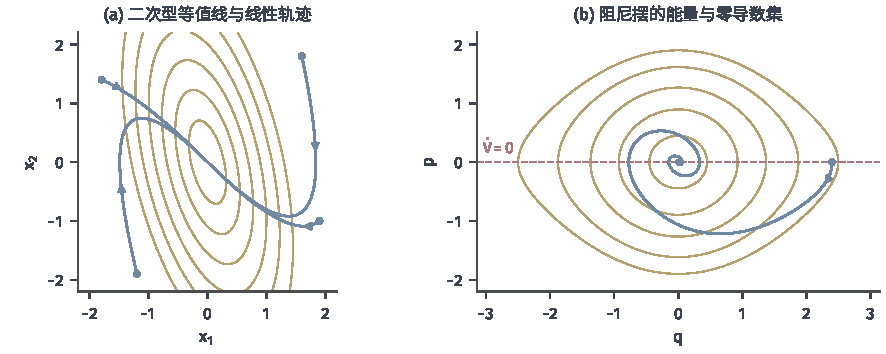
\includegraphics[width=150mm]{figures/03-optimization-evolution-and-signals/02-processes-and-trajectory-evolution/matplotlib/ode-lyapunov-levels/figure.pdf}
  \caption{Lyapunov函数的等值线与轨迹。(a)线性系统$\bm A=\begin{bmatrix}0&1\\-2&-3\end{bmatrix}$，黄色椭圆是示例~\ref{ex:ode-lyapunov-equation}中$V=\bm x^\top\bm P\bm x$的等值线，四条蓝色轨迹计算到$t=8$，每次穿过椭圆都由外向内。(b)阻尼摆$\dot q=p$，$\dot p=-\sin q-0.5p$，黄色曲线是机械能$V=p^2/2+1-\cos q$的等值线，红色虚线是零导数集$p=0$；蓝色轨迹从$(2.4,0)$出发（$V\approx1.737$），虽从零导数集上起步，却立刻被推离，$t=30$时$V$约为$10^{-6}$。}
  \label{fig:ode-lyapunov-levels}
\end{figure*}

图~\ref{fig:ode-lyapunov-levels}(b)画出这个论证。轨迹每次穿过$p=0$时能量暂时不减，但它不能沿着$p=0$走下去，因为那里的向量场$(0,-\sin q)$在$q\neq0$时竖直地指离这条直线。能量的单调性先把轨迹限制在一个紧区域里，动力学再排除那些不能持续停留的零导数点。若把整个$E$都称为“最终状态”，就漏掉了论证中最关键的一步。

无阻尼时$c=0$，$\dot V\equiv0$，能量守恒，$E=\Omega$，最大不变集是整个$\Omega$：LaSalle原理只给出平凡的结论。这时最低点稳定（能量的子水平集是围绕它的小闭曲线，由定理~\ref{thm:ode-lyapunov}的(1)），却不吸引，轨迹沿等能量的闭曲线永远摆动。

\paragraph{梯度流：下降、驻点与收敛}
优化中最常见的连续时间动力学是\term{梯度流}
\begin{equation}
  \dot{\bm x}=-\nabla F(\bm x),
  \label{eq:ode-gradient-flow}
\end{equation}
其中$F:\mathbb R^d\to\mathbb R$连续可微且$\nabla F$局部Lipschitz。目标函数本身就是候选的Lyapunov函数：$\dot F=\nabla F^\top(-\nabla F)=-\|\nabla F\|_2^2\leq0$，下降速率恰是梯度长度的平方。积分得
\[
  \int_0^T\|\nabla F(\bm x(t))\|_2^2\,\mathrm dt=F(\bm x_0)-F(\bm x(T)).
\]
若$F$有下界，左端对一切$T$有统一的上界，所以梯度在大部分时间里都很小。

由此能推出多少，取决于额外条件。若子水平集$\{F\leq F(\bm x_0)\}$有界，它就是紧的正向不变集，LaSalle原理（取$V=F$）说明轨迹趋于$E=\{\nabla F=\bm0\}$中的最大不变集；驻点都是平衡点，平衡点组成的集合本身不变，所以轨迹趋于驻点组成的集合。这个结论没有说轨迹收敛到某一个驻点，对一般光滑函数这一点确实可能不成立。若子水平集无界，连趋于驻点也不能保证：一维的$F(x)=e^{-x}$下界为零但没有最小点，梯度流$\dot x=e^{-x}$的解$x(t)=\log(e^{x_0}+t)$趋于无穷，$F$下降到$0$，状态却没有极限。下降有下界，不等于状态收敛。

强凸性给出最干净的结论。设存在$\mu>0$使$\langle\nabla F(\bm x)-\nabla F(\bm y),\bm x-\bm y\rangle\geq\mu\|\bm x-\bm y\|_2^2$对一切$\bm x,\bm y$成立，$\bm x^\ast$为唯一的最小点。则
\[
  \frac{\mathrm d}{\mathrm dt}\frac12\|\bm x-\bm x^\ast\|_2^2=-\langle\nabla F(\bm x)-\nabla F(\bm x^\ast),\bm x-\bm x^\ast\rangle\leq-\mu\|\bm x-\bm x^\ast\|_2^2,
\]
于是$\|\bm x(t)-\bm x^\ast\|_2\leq e^{-\mu t}\|\bm x_0-\bm x^\ast\|_2$，全局指数稳定。在非退化的鞍点处，Hessian矩阵有负特征值，梯度流的线性化$-\nabla^2F$有正特征值，由定理~\ref{thm:ode-linearization}，鞍点不稳定。梯度下降是梯度流的显式Euler离散，离散算法的步长条件与收敛速率在第~\ref{chap:opt-smooth}章研究；连续流的结论不能代替离散算法的定理，两者的关系正是第~\ref{sec:ode-numerics}节的数值离散问题。

\paragraph{周期轨道与极限环}
长期行为不一定是趋于平衡点。若非常值解满足$\bm x(t+T)=\bm x(t)$对一切$t$成立（$T>0$），它的轨迹是一条闭曲线，称为周期轨道。无阻尼摆的等能量曲线都是周期轨道，但它们一条挨着一条，邻近的轨迹不会靠过来。另一类周期轨道会吸引周围的轨迹，称为\term{极限环}（limit cycle）。van der Pol方程
\[
  \dot x=y,\qquad\dot y=\mu(1-x^2)y-x,\qquad\mu>0
\]
是典型例子。看能量$E=(x^2+y^2)/2$：$\dot E=\mu(1-x^2)y^2$，在$|x|<1$的带子里向系统注入能量，在$|x|>1$处耗散能量。小的振荡被放大，大的振荡被削弱，二者在一条闭曲线上平衡。图~\ref{fig:ode-limit-cycle-bifurcation}(a)显示，从原点附近和远处出发的轨迹都趋于同一条闭曲线，它们的$\omega$极限集就是这条极限环，而唯一的平衡点原点不稳定。对平面系统，Poincaré--Bendixson定理说明：若一条正向有界轨迹的$\omega$极限集不含平衡点，它就是一条周期轨道\scite{math-khalil2002nonlinear}。维数更高时，长期行为可以复杂得多，离散时间中的敏感依赖已在第~\ref{chap:discrete-dynamical-systems}章出现。

\begin{figure*}[htbp]
  \centering
  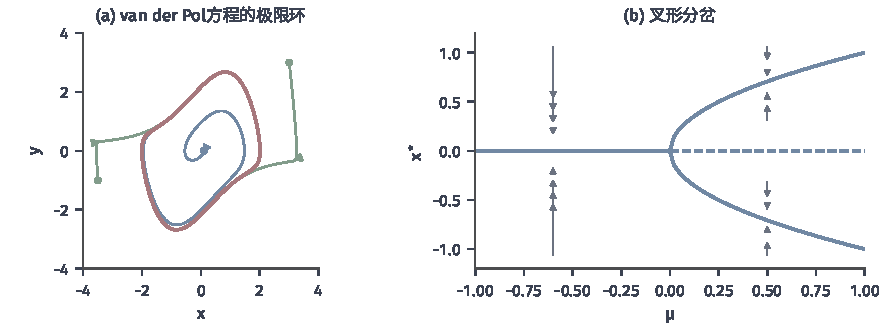
\includegraphics[width=150mm]{figures/03-optimization-evolution-and-signals/02-processes-and-trajectory-evolution/matplotlib/ode-limit-cycle-bifurcation/figure.pdf}
  \caption{平衡点之外的长期行为与参数变化。(a)van der Pol方程$\dot x=y$，$\dot y=(1-x^2)y-x$：从$(0.1,0)$（蓝）以及$(3,3)$、$(-3.5,-1)$（绿）出发的轨迹计算到$t=30$，都趋于红色的极限环。(b)方程$\dot x=\mu x-x^3$的平衡点随参数$\mu$的变化：实线为稳定平衡点，虚线为不稳定平衡点，灰色箭头是$\mu=-0.6$与$\mu=0.5$时状态的运动方向。}
  \label{fig:ode-limit-cycle-bifurcation}
\end{figure*}

\paragraph{参数变化与局部分岔}
向量场含参数时，平衡点及其稳定性会随参数改变。最简单的例子是$\dot x=\mu x-x^3$。$\mu<0$时唯一的平衡点是原点，线性化$\mu<0$，稳定。$\mu>0$时原点的线性化$\mu>0$，变得不稳定，同时出现两个新的平衡点$\pm\sqrt\mu$，其线性化为$\mu-3\mu=-2\mu<0$，都是稳定的。图~\ref{fig:ode-limit-cycle-bifurcation}(b)中平衡点的分支像一把叉子，称为叉形分岔。转变发生在$\mu=0$，那里线性化的特征值穿过零，正是线性化判据失效的临界情形。

van der Pol方程在原点的线性化是$\begin{bmatrix}0&1\\-1&\mu\end{bmatrix}$，特征值$\bigl(\mu\pm\sqrt{\mu^2-4}\bigr)/2$。$\mu$从负变正时，一对复特征值从左向右穿过虚轴，原点由稳定焦点变为不稳定焦点，同时出现极限环。特征值穿过虚轴的位置决定了分岔的类型：穿过零点产生新的平衡点，成对的复特征值穿过虚轴产生周期轨道。完整的分岔理论需要中心流形等工具，本书不展开；这两个低维例子说明，线性化判据的临界情形往往正是定性行为发生改变的地方。

\subsection{持续输入下的轨迹响应}
\label{sec:ode-input-response}

初值误差只在开始时注入一次，稳定系统会逐渐把它忘掉。输入则可以在每个时刻持续地推动状态：暖气的功率一直偏大，房间就一直偏热，不会因为系统“稳定”而回到原来的温度。本小节估计持续输入留下的状态范围，区分哪些部分会被遗忘、哪些部分会保留。

\paragraph{线性系统：初态记忆与输入留下的范围}
设$\bm A$为Hurwitz矩阵，由定理~\ref{thm:ode-linear-spectral-stability}有常数$M\geq1$、$\alpha>0$使$\|e^{t\bm A}\|\leq Me^{-\alpha t}$。对常数变易公式~\eqref{eq:ode-lti-variation}两项分别取范数，得
\begin{equation}
  \|\bm x(t)\|_2\leq Me^{-\alpha(t-t_0)}\|\bm x_0\|_2+M\|\bm B\|\int_{t_0}^te^{-\alpha(t-s)}\|\bm u(s)\|_2\,\mathrm ds.
  \label{eq:ode-linear-input-bound}
\end{equation}
若$\|\bm u(s)\|_2\leq U$，第二项不超过$\frac{M\|\bm B\|U}{\alpha}\bigl(1-e^{-\alpha(t-t_0)}\bigr)$。第一项是初态的记忆，按指数衰减；第二项是输入的累计，最终不超过$M\|\bm B\|U/\alpha$。所以有界输入产生有界状态，状态最终落入半径约为$M\|\bm B\|U/\alpha$的范围，与初态无关。两组初值与输入之差满足同一个线性方程，把上式中的状态、初值和输入分别换成差，就得到两条轨迹的比较界：初值差被遗忘，输入差留下。

以温度模型为例，取示例~\ref{ex:ode-periodic-heating}的周期加热$u(t)=0.4+0.2\sin(0.5t)$。对偏差$x-2$应用式~\eqref{eq:ode-linear-input-bound}，$M=1$、$\alpha=0.2$、$U=0.2$，得
\[
  |x(t)-2|\leq e^{-0.2t}|x_0-2|+\bigl(1-e^{-0.2t}\bigr),
\]
最终范围是$[1,3]$。图~\ref{fig:ode-input-response}显示，从$x_0=0$与$x_0=4$出发的两条轨迹在约$20$分钟后几乎重合，都贴近示例~\ref{ex:ode-periodic-heating}算出的稳态振荡$2+0.371\sin(0.5t-1.19)$。实际振幅$0.371$远小于界给出的$1$：界只用了输入的大小，没有用到输入在快速摆动、正负部分相互抵消这一点。

\begin{figure}[htbp]
  \centering
  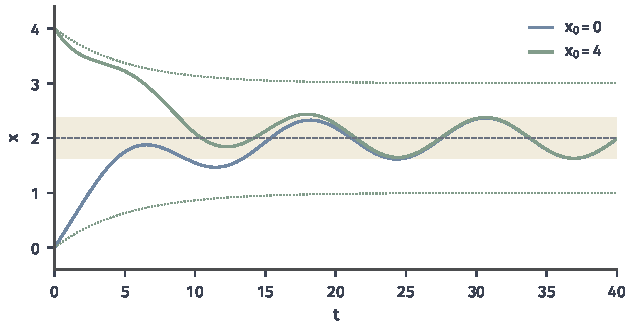
\includegraphics[width=107mm]{figures/03-optimization-evolution-and-signals/02-processes-and-trajectory-evolution/matplotlib/ode-input-response/figure.pdf}
  \caption{持续输入下的温度响应。方程$\dot x=-0.2x+u$，$u(t)=0.4+0.2\sin(0.5t)$。蓝、绿实线分别从$x_0=0$与$x_0=4$出发；同色点线是式~\eqref{eq:ode-linear-input-bound}给出的上下界$2\pm\bigl(e^{-0.2t}|x_0-2|+1-e^{-0.2t}\bigr)$；浅黄带是稳态振荡的范围$2\pm0.371$，灰色虚线为平均平衡值$2$。}
  \label{fig:ode-input-response}
\end{figure}

恒定的偏差最能说明“稳定不消除持续扰动”。若加热量固定偏多$\delta u$，平衡点从$u/\lambda$移到$(u+\delta u)/\lambda$，稳态偏差为$\delta u/\lambda$；$\lambda=0.2$时是$5\,\delta u$。初值的影响以速率$0.2$衰减，这个偏差却一直存在。消除它需要根据测得的温度调整加热量，那是反馈控制的任务。

\paragraph{非线性系统：含输入项的Lyapunov不等式}
非线性系统没有常数变易公式，但Lyapunov函数的方法可以把输入写进下降条件。设$\dot{\bm x}=\bm g(\bm x,\bm u)$，$\bm g(\bm0,\bm0)=\bm0$，并有连续可微的$V$与常数$c_1,c_2,c_3,\gamma>0$，使对一切$\bm x$与输入值$\bm v$，
\begin{equation}
  c_1\|\bm x\|_2^2\leq V(\bm x)\leq c_2\|\bm x\|_2^2,\qquad
  \nabla V(\bm x)^\top\bm g(\bm x,\bm v)\leq-c_3\|\bm x\|_2^2+\gamma\|\bm v\|_2^2.
  \label{eq:ode-iss-lyapunov}
\end{equation}
第二个条件说：状态大时$V$下降，输入大时$V$可以上升，上升的幅度由增益$\gamma$控制。

\begin{theorem}[含输入项的Lyapunov估计]
  \label{thm:ode-iss-bound}
  在条件~\eqref{eq:ode-iss-lyapunov}下，设输入$\bm u$可测且$\|\bm u(t)\|_2\leq U$，$\bm g$关于状态局部Lipschitz并满足Carathéodory条件。则每条解对全部$t\geq t_0$存在，并且
  \[
    \|\bm x(t)\|_2^2\leq\frac{c_2}{c_1}e^{-(c_3/c_2)(t-t_0)}\|\bm x_0\|_2^2+\frac{\gamma c_2}{c_1c_3}U^2.
  \]
\end{theorem}

\begin{proof}
  令$v(t)=V(\bm x(t))$，它沿绝对连续的解几乎处处可导，由条件~\eqref{eq:ode-iss-lyapunov}，$\dot v\leq-c_3\|\bm x\|_2^2+\gamma U^2\leq-(c_3/c_2)v+\gamma U^2$。记$k=c_3/c_2$，则$\frac{\mathrm d}{\mathrm dt}\bigl(e^{k(t-t_0)}v\bigr)\leq\gamma U^2e^{k(t-t_0)}$，积分得$v(t)\leq e^{-k(t-t_0)}v(t_0)+\gamma U^2/k$。再用$c_1\|\bm x\|_2^2\leq v$与$v(t_0)\leq c_2\|\bm x_0\|_2^2$即得所述不等式。它在解的存在区间上成立，说明解留在一个有界集合中，由定理~\ref{thm:ode-escape}，解对全部$t\geq t_0$存在。
\end{proof}

满足这类条件的系统称为\term{输入到状态稳定}（input-to-state stable, ISS）的一种二次形式：初态的影响按指数衰减，输入只留下与其大小成比例的最终范围。例如$\dot x=-x-x^3+u$，取$V=x^2/2$，则$\dot V=-x^2-x^4+xu\leq-x^2+xu\leq-\tfrac12x^2+\tfrac12u^2$，最后一步用了$xu\leq\tfrac12x^2+\tfrac12u^2$。于是$c_1=c_2=c_3=\gamma=\tfrac12$，定理给出$\limsup_{t\to\infty}|x(t)|\leq U$。

无输入时稳定，不等于有输入时有界。$\dot x=-x+x^2u$在$u\equiv0$时原点全局指数稳定；可是取恒定输入$u\equiv1$、$x_0=2$，方程变成$\dot x=x(x-1)$，解为$x(t)=1/(1-e^t/2)$，在$t=\log2$时爆炸。问题在于输入通过$x^2$进入方程，状态越大，输入的作用越强，条件~\eqref{eq:ode-iss-lyapunov}无法成立。本小节分析的是给定系统对给定输入的响应；如何设计依赖状态的输入，使闭环满足这类条件，是反馈稳定化的问题，可参考\BookChapterRef{chap:control-theory}{卷五“策略的实现与轨迹控制”章}。
